\documentclass[prd, superscriptaddress, tightenlines, longbibliography, nofootinbib, eqsecnum, amsfonts, amsmath, floatfix, twocolumn, notitlepage]{revtex4-2}
\pdfoutput=1
\usepackage{ftnxtra}
%\usepackage{footmisc}
\usepackage[utf8]{inputenc}
\usepackage{mathrsfs}
\usepackage{euscript}
\usepackage{graphics}
\usepackage{graphicx}
\usepackage{amsmath}
\usepackage{amssymb}
\usepackage{gensymb}
\usepackage{tabularx}
\usepackage{subfigure}
%\usepackage{subcaption}
\usepackage{bm}
\usepackage[usenames,dvipsnames,svgnames,table]{xcolor}
\definecolor{linkcolor}{rgb}{0.6,0,0}
\definecolor{citecolor}{rgb}{0,0,0.75}
\definecolor{urlcolor}{rgb}{0.12,0.46,0.7}
\usepackage{xspace}
\usepackage{wasysym}
\usepackage{times}
\usepackage{appendix}
\usepackage{comment}
\usepackage{lipsum}
\usepackage[nolist,nohyperlinks]{acronym}
\usepackage{float}
\usepackage{simplewick}
\usepackage{natbib, ifthen}
\usepackage[breaklinks, colorlinks, urlcolor=urlcolor, linkcolor=linkcolor,citecolor=citecolor,pdfencoding=auto]{hyperref}
%\usepackage{longtable}
%\usepackage{booktabs} % for tables
\usepackage{listings}
\interfootnotelinepenalty=1000000
\newcommand{\apjs} {Astrophys. J. Suppl.}
\usepackage{caption}

\newcommand{\orcid}[1]{{\sc ORCiD:} \href{https://orcid.org/#1}{#1}}
\newcommand{\orcidacronym}[2]{\href{https://orcid.org/#2}{#1}}
\newcommand{\ALorcid}{\orcidacronym{AL}{0000-0001-5927-6667}}

\newcommand{\la}{\langle}
\newcommand{\ra}{\rangle}

\newcommand{\onesig}[1]{(68\%, \text{#1})}
\newcommand{\twosig}[1]{(95\%, \text{#1})}
\newcommand{\twoonesig}[3]{
\begin{equation}
\left.
 \begin{aligned}
#1 \\ #2
 \end{aligned}
\ \right\} \ \ \mbox{\text{#3}}
\end{equation}
}
\newcommand{\twotwosig}[3]{
\begin{equation}
\left.
 \begin{aligned}
#1 \\ #2
 \end{aligned}
\ \right\} \ \ \mbox{95\%, \text{#3}}
\end{equation}
}


\newcommand{\fsky}{f_{\rm sky}}


\providecommand{\planck}{\textit{Planck}}
\providecommand{\Planck}{\planck}
\newcommand{\camspec}{{\tt CamSpec}}
\newcommand{\plik}{{\tt Plik}}
\newcommand{\commander}{{\tt Commander}}
\newcommand{\mspec}{{\tt MSPEC}}
\newcommand{\smica}{{\tt SMICA}}

\newcommand{\MCNzero}{\textrm{MC-}N^{(0)}}
\newcommand{\RDNzero}{\textrm{RD-}N^{(0)}}
\newcommand{\RDNone}[0]{\textrm{RD-}N^{(1)}}
\newcommand{\xpRDNone}[0]{\textrm{xpRD-}N^{(1)}}
\newcommand{\MCNone}[0]{\textrm{MC-}N^{(1)}}

\newcommand{\CFHTLENS}{CFHTLenS}
\newcommand{\meanchisquare}{\overline{\chi^2}}

\newcommand{\mksym}[1]{\ifmmode {\rm #1}\else #1\fi}
\newcommand{\dataplus}{{+}}
\newcommand{\WP}{\mksym{WP}}
\newcommand{\highL}{\mksym{highL}}
\newcommand{\BAO}{\mksym{BAO}}
\newcommand{\lensing}{\mksym{lensing}}
\newcommand{\ext}{\mksym{ext}}
\newcommand{\planckonly}{\planck}
\newcommand{\TT}{\mksym{TT}}
\newcommand{\TTTEEE}{\mksym{TT,TE,EE}}
\newcommand{\planckTTonly}{\planck\ \TT}
\newcommand{\planckTTTEEEonly}{\planck\ \TTTEEE}
\newcommand{\lowTEB}{\mksym{lowP}}
\newcommand{\lowEB}{\mksym{lowP}}
\newcommand{\WMAPTEB}{\lowTEB\dataplus\mksym{WP}}
\newcommand{\lowTP}{\mksym{lowT,P}}
\newcommand{\planckTT}{\planckTTonly\dataplus\lowTEB}
\newcommand{\planckall}{\planckTTTEEEonly\dataplus\lowTEB}
\newcommand{\planckTTBAO}{\planckTT\dataplus\BAO}
\newcommand{\planckTTlensing}{\planckTT\dataplus\lensing}
\newcommand{\planckallBAO}{\planckall\dataplus\BAO}
\newcommand{\planckalllensing}{\planckall\dataplus\lensing}
\newcommand{\planckTTlensext}{\planckTT\dataplus\lensing\dataplus\ext}
\newcommand{\datalabel}[1]{#1}

\newcommand{\shortTT}{\TT\dataplus\lowTEB}
\newcommand{\shortall}{\TTTEEE\dataplus\lowTEB}

\newcommand{\HighL}{\highL}

\newcommand{\As}{A_{\rm s}}
\newcommand{\At}{A_{\rm t}}
\newcommand{\nt}{n_{\rm t}}
\newcommand{\ns}{n_{\rm s}}
\newcommand{\lcdm}{{$\rm{\Lambda CDM}$}}
\newcommand{\rpivot}{r_{0.05}}
\newcommand{\rzerotwo}{r_{0.002}}
\newcommand{\Alens}{A_{\rm L}}
\newcommand{\Aphiphi}{A_{\rm L}^{\phi\phi}}
\newcommand{\omegak}{\Omega_K}
\newcommand{\omegal}{\Omega_\Lambda}
\newcommand{\alphaiso}{\alpha}

%\newcommand{\nrun}{n_{\text{run}}}
\newcommand{\thetaMC}{\theta_{\rm MC}}
\newcommand{\nrun}{d \ns / d\ln k}
\newcommand{\nrunfrac}{\frac{d \ns}{d\ln k}}
\newcommand{\zre}{z_{\text{re}}}
\newcommand{\yhe}{Y_{\text{P}}}
\newcommand{\ypbbn}{Y_{\text{P}}^{\rm BBN}}
\newcommand{\zeq}{z_{\text{eq}}}
\newcommand{\nnu}{N_{\rm eff}}
\newcommand{\neff}{\nnu}
\newcommand{\mnu}{\sum m_\nu}
\newcommand{\sumnu}{\sum m_\nu}
\newcommand{\mnusterile}{m_{\nu,\, \mathrm{sterile}}^{\mathrm{eff}}}
\newcommand{\meffsterile}{\mnusterile}
\newcommand{\Tactive}{T_{\mathrm{a}}}
\newcommand{\Tsterile}{T_{\mathrm{s}}}
\newcommand{\msthermal}{m_{\rm sterile}^{\rm thermal}}
\newcommand{\msDW}{m_{\rm sterile}^{\rm DW}}

\newcommand{\zdrag}{z_{\rm drag}}
\newcommand{\rdrag}{r_{\rm drag}}
\newcommand{\zstar}{z_{\ast}}
\newcommand{\rstar}{r_{\ast}}
\newcommand{\rs}{r_{\rm s}}
\newcommand{\thetastar}{\theta_{\ast}}
\newcommand{\DAstar}{D_{\rm A}}
\newcommand{\keq}{k_{\rm eq}}
\newcommand{\Ailensbestfit}{A_i^{\mbox{\scriptsize{theory}}}}
\newcommand{\Alensbestfit}{A^{\mbox{\scriptsize{theory}}}}
\newcommand{\DVBAO}{D_{\rm V}}
\newcommand{\DA}{D_{\rm A}}


%\newcommand{\zeq}{z_{\rm eq}}


\newcommand{\fixme}[1]{{\color{Red}{ FIXME: #1}}}
\newcommand{\quietfixme}[1]{{\color{Red} #1}}
\newcommand{\notate}[1]{{\color{olive} NOTE: #1}}

\newcommand{\fnl}{\ensuremath{f_{\text{NL}}}}

\newcommand{\taunl}{\ensuremath{{\tau_{\text{NL}}}}}

\newcommand{\gnl}{\ensuremath{g_{\text{NL}}}}

% tauNL-estimator
\newcommand{\htaunl}{\ensuremath{{\hat{\tau}_{\rm NL}}}}


\newcommand{\fnlloc}{f^{\rm local}_{\rm NL}}
\newcommand{\fnleqi}{f^{\rm equil}_{\rm NL}}

\providecommand{\Planck}{\textit{Planck}}
\providecommand{\planck}{\Planck}
\newcommand{\covinvT}{\bar{\Theta}}
\newcommand{\Ltemp}{\tilde{T}}
\newcommand{\lensedC}{\tilde{C}}
\newcommand{\Lmin}{{L_{\rm min}}}

%\providecommand{\lea}{\lesssim}
%\providecommand{\gea}{\gtrsim}
\providecommand{\lea}{\la}
\providecommand{\gea}{\ga}


\providecommand{\alt}{\lea}
\providecommand{\agt}{\gea}
\providecommand{\text}[1]{\rm{#1}}



\newcommand{\Msun}{M_\odot}
\newcommand{\tot}{{\text{tot}}}
\newcommand{\Mpc}{\text{Mpc}}
\newcommand{\half}{{\textstyle \frac{1}{2}}}
\newcommand{\third}{{\textstyle \frac{1}{3}}}
\newcommand{\numfrac}[2]{{\textstyle \frac{#1}{#2}}}
\renewcommand{\d}{\text{d}}
\newcommand{\grad}{\nabla}
\newcommand{\km}{{\rm{\,km\,}}}

\newcommand{\Hunit}{\text{km}\,\text{s}^{-1}\,\Mpc^{-1}}
\newcommand{\Gyr}{{\rm Gyr}}
\providecommand{\muK}{\mu{\rm K}}
\providecommand{\arcmin}{{\rm arcmin}}
\newcommand{\muKarcmin}{\,\muK\,\arcmin}
\newcommand{\muKsq}{(\mu\rm{K})^2}
\newcommand{\lmax}{l_{\text{max}}}
\newcommand{\lmin}{l_{\text{min}}}

\newcommand{\mpl}{m_{\text{Pl}}}
\newcommand{\eV}{\,\text{eV}}
\newcommand{\MeV}{\,\text{MeV}}
\newcommand{\GeV}{\,\text{GeV}}


\providecommand{\Omk}{\Omega_K}
\providecommand{\Oml}{\Omega_{\Lambda}}
\providecommand{\Omtot}{\Omega_{\mathrm{tot}}}
\providecommand{\Omb}{\Omega_{\mathrm{b}}}
\providecommand{\Omc}{\Omega_{\mathrm{c}}}
\providecommand{\Omm}{\Omega_{\mathrm{m}}}
\providecommand{\omb}{\omega_{\mathrm{b}}}
\providecommand{\omc}{\omega_{\mathrm{c}}}
\providecommand{\omm}{\omega_{\mathrm{m}}}
\providecommand{\Omdm}{\Omega_{\mathrm{DM}}}
\providecommand{\Omnu}{\Omega_{\nu}}

\providecommand{\CAMB}{{\tt camb}}
\providecommand{\GetDist}{{\tt GetDist}}
\providecommand{\Cobaya}{{\tt Cobaya}}


\providecommand{\COSMOMC}{{\tt CosmoMC}}
\providecommand{\CMBFAST}{{\tt cmbfast}}
\providecommand{\COSMICS}{{\tt Cosmics}}
\providecommand{\CLASS}{{\tt class}}
\providecommand{\CMBEASY}{{\tt cmbeasy}}
\providecommand{\LCDM}{{$\rm{\Lambda CDM}$}}
\providecommand{\COSMOREC}{{\tt CosmoRec}}
\providecommand{\HYREC}{{\tt HyRec}}
\providecommand{\RECFAST}{{\tt recfast}}
\providecommand{\HALOFIT}{{\tt halofit}}
\providecommand{\AlterBBN}{{\tt AlterBBN}}
\providecommand{\MontePython}{{\tt Monte Python}}
\providecommand{\HEALpix}{{\tt HEALpix}}


\newcommand{\begm}{\begin{pmatrix}}
\newcommand{\enm}{\end{pmatrix}}
\newcommand{\threej}[6]{{\begm #1 & #2 & #3 \\ #4 & #5 & #6 \enm}}
\newcommand{\threejz}[3]{{\begm #1 & #2 & #3 \\ 0 & 0 & 0 \enm}}

\newcommand\ba{\begin{eqnarray}}
\newcommand\ea{\end{eqnarray}}
\newcommand\bea{\begin{eqnarray}}
\newcommand\eea{\end{eqnarray}}

\newcommand\be{\begin{equation}}
\newcommand\ee{\end{equation}}




\newcommand{\valpha}{{\boldsymbol{\alpha}}}
\newcommand{\vgrad}{{\boldsymbol{\nabla}}}
\newcommand{\vpsi}{\mathbf{\psi}}
\newcommand{\vTheta}{\mathbf{\Theta}}
\newcommand{\vtheta}{\boldsymbol{\theta}}
\newcommand{\vdelta}{\boldsymbol{\delta}}
\newcommand{\vell}{{\boldsymbol{\ell}}}


%%%%% statistics %%%%%%%%%%%%

%Variance
\providecommand{\var}{\text{var}}
%covariance
\providecommand{\cov}{\text{cov}}

\providecommand{\Tr}{\text{Tr}}
%likelihood

%integration
\newcommand{\ud}{{\rm d}}


%%%%%%% Matrices %%%%%%%%%%
\newcommand{\mA}{\bm{A}}
\newcommand{\mB}{\bm{B}}
\newcommand{\mC}{\bm{C}}
\newcommand{\mD}{\bm{D}}
\newcommand{\mE}{\bm{E}}
\newcommand{\mF}{\bm{F}}
\newcommand{\mG}{\bm{G}}
\newcommand{\mH}{\bm{H}}
\newcommand{\mI}{\bm{I}}
\newcommand{\mJ}{\bm{J}}
\newcommand{\mK}{\bm{K}}
\newcommand{\mL}{\bm{L}}
\newcommand{\mM}{\bm{M}}
\newcommand{\mN}{\bm{N}}
\newcommand{\mO}{\bm{O}}
\newcommand{\mP}{\bm{P}}
\newcommand{\mQ}{\bm{Q}}
\newcommand{\mR}{\bm{R}}
\newcommand{\mS}{\bm{S}}
\newcommand{\mT}{\bm{T}}
\newcommand{\mU}{\bm{U}}
\newcommand{\mV}{\bm{V}}
\newcommand{\mW}{\bm{W}}
\newcommand{\mX}{\bm{X}}
\newcommand{\mY}{\bm{Y}}
\newcommand{\mZ}{\bm{Z}}

\newcommand{\mLambda}{\bm{\Lambda}}
\newcommand{\mzero}{\bm{0}}

%%%%%%%% Vectors %%%%%%%%%%

\newcommand{\boldvec}[1]{{\mbox{\boldmath{$#1$}}}}

\newcommand{\vA}{\boldvec{A}}
\newcommand{\vB}{\boldvec{B}}
\newcommand{\vC}{\boldvec{C}}
\newcommand{\vD}{\boldvec{D}}
\newcommand{\vE}{\boldvec{E}}
\newcommand{\vF}{\boldvec{F}}
\newcommand{\vG}{\boldvec{G}}
\newcommand{\vH}{\boldvec{H}}
\newcommand{\vI}{\boldvec{I}}
\newcommand{\vJ}{\boldvec{J}}
\newcommand{\vK}{\boldvec{K}}
\newcommand{\vL}{\boldvec{L}}
\newcommand{\vM}{\boldvec{M}}
\newcommand{\vN}{\boldvec{N}}
\newcommand{\vO}{\boldvec{O}}
\newcommand{\vP}{\boldvec{P}}
\newcommand{\vQ}{\boldvec{Q}}
\newcommand{\vR}{\boldvec{R}}
\newcommand{\vS}{\boldvec{S}}
\newcommand{\vT}{\boldvec{T}}
\newcommand{\vU}{\boldvec{U}}
\newcommand{\vV}{\boldvec{V}}
\newcommand{\vW}{\boldvec{W}}
\newcommand{\vX}{\boldvec{X}}
\newcommand{\vY}{\boldvec{Y}}
\newcommand{\vZ}{\boldvec{Z}}

\newcommand{\va}{\boldvec{a}}
\newcommand{\vb}{\boldvec{b}}
\newcommand{\vc}{\boldvec{c}}
\newcommand{\vd}{\boldvec{d}}
\newcommand{\ve}{\boldvec{e}}
\newcommand{\vf}{\boldvec{f}}
\newcommand{\vg}{\boldvec{g}}
\newcommand{\vh}{\boldvec{h}}
\newcommand{\vi}{\boldvec{i}}
\newcommand{\vj}{\boldvec{j}}
\newcommand{\vk}{\boldvec{k}}
\newcommand{\vl}{\boldvec{l}}
\newcommand{\vm}{\boldvec{m}}
\newcommand{\vn}{\boldvec{n}}
\newcommand{\vo}{\boldvec{o}}
\newcommand{\vp}{\boldvec{p}}
\newcommand{\vq}{\boldvec{q}}
\providecommand{\vr}{\boldvec{r}}
\newcommand{\vs}{\boldvec{s}}
\newcommand{\vt}{\boldvec{t}}
\newcommand{\vu}{\boldvec{u}}
\newcommand{\vv}{\boldvec{v}}
\newcommand{\vw}{\boldvec{w}}
\newcommand{\vx}{\boldvec{x}}
\newcommand{\vy}{\boldvec{y}}
\newcommand{\vz}{\boldvec{z}}

\newcommand{\cla}{\mathcal{A}}
\newcommand{\clb}{\mathcal{B}}
\newcommand{\clc}{\mathcal{C}}
\newcommand{\cld}{\mathcal{D}}
\newcommand{\cle}{\mathcal{E}}
\newcommand{\clf}{\mathcal{F}}
\newcommand{\clg}{\mathcal{G}}
\newcommand{\clh}{\mathcal{H}}
\newcommand{\cli}{\mathcal{I}}
\newcommand{\clj}{\mathcal{J}}
\newcommand{\clk}{\mathcal{K}}
\newcommand{\cll}{\mathcal{L}}
\newcommand{\clm}{\mathcal{M}}
\newcommand{\cln}{\mathcal{N}}
\newcommand{\clo}{\mathcal{O}}
\newcommand{\clp}{\mathcal{P}}
\newcommand{\clq}{\mathcal{Q}}
\newcommand{\clr}{\mathcal{R}}
\newcommand{\cls}{\mathcal{S}}
\newcommand{\clt}{\mathcal{T}}
\newcommand{\clu}{\mathcal{U}}
\newcommand{\clv}{\mathcal{V}}
\newcommand{\clw}{\mathcal{W}}
\newcommand{\clx}{\mathcal{X}}
\newcommand{\cly}{\mathcal{Y}}
\newcommand{\clz}{\mathcal{Z}}



\newcommand{\vnhat}{\hat{\vn}}
\newcommand{\vrhat}{\hat{\vr}}
\newcommand{\vkhat}{\hat{\vk}}

\providecommand{\ltsima}{\lea}
\providecommand{\gtsima}{\gea}
\providecommand{\simlt}{\lea}
\providecommand{\simgt}{\gea}


\newcommand{\elec}{{\rm e}}
\newcommand{\neutron}{{\rm n}}

%
%-------------------------------------------------------------------

\defcitealias{PL2018}{PL2018}
\newcommand{\PL}{\citetalias{PL2018}\xspace}

\defcitealias{Carron:2022eyg}{PL4}
\newcommand{\NPIPE}{\citetalias{Carron:2022eyg}\xspace}


\newcommand{\Simons}[0]{\emph{Simons Observatory}}
\newcommand{\isdraft}[1]{#1}
%\newcommand{\isdraft}[1]{}

%\newcommand{\JC}[1]{{\isdraft{\color{red}{#1}\color{black}}}}
\newcommand{\JC}[1]{\color{purple}{{JC:#1}}\color{black}\xspace}
\newcommand{\LL}[1]{{\color{orange}{LL: #1}}}

\newcommand{\plancklens}{\texttt{plancklens}}
\newcommand{\Cov}[0]{ {\rm{Cov}} }
\newcommand{\LM}[0]{{LM}}
\newcommand{\bL}[0]{\ensuremath{\bm{L}}\xspace}
% \newcommand{\bl}[0]{\ensuremath{\boldmath{\ell}}\xspace}
% \newcommand{\ba}[0]{\ensuremath{\bm{\alpha}}\xspace}


\newcommand{\eff}{\textrm{eff}}
\newcommand{\vecx}{\mathbf{x} }
\newcommand{\fid}{\rm fid}
\newcommand{\g}{g}
\newcommand{\R}{\mathcal{R}}
\newcommand{\filt}{\rm filt}
\newcommand{\MC}{\text{MC}}
\newcommand{\fpatch}{f_{A,L}}
\newcommand{\vecell}{ {\boldsymbol  \ell}}
%\newcommand{\fsky}{f_{\rm sky}}

\newcommand{\ellsky}{\ell_{\rm sky}}
\newcommand{\msky}{m_{\rm sky}}

\newcommand{\av}[1]{\left \langle #1\right\rangle}
\newcommand{\bs}[1]{\boldsymbol{#1}}
\newcommand{\Tfiras}{T_{\text{\sc FIRAS}}}
\newcommand{\Rtt}[0]{ {R^{TT}} }
\newcommand{\Rpt}[0]{ {R^{\phi T}} }
\newcommand{\TWF}[0]{T^{\rm WF}}
\newcommand{\TWFd}[0]{T^{\rm WF, \dagger}}

\renewcommand{\thefootnote}{\arabic{footnote}}

\begin{document}

\title{Extracting Cluster Information from small scale CMB-lensing}

\newcommand{\Geneve}{Universit\'e de Gen\`eve, D\'epartement de Physique Th\'eorique et CAP, 24 Quai Ansermet, CH-1211 Gen\`eve 4, Switzerland}
\newcommand{\IISER}{Department of Physics, Indian Institute of Science Education and Research, Pune 411008, India}
\newcommand{\RRI}{Raman Research Institute, C. V. Raman Avenue, Sadashivanagar, Bengaluru 560080, India}
\newcommand{\ICTP}{Instituto de F\'isica Te\'orica da Universidade Estadual Paulista and ICTP South American Institute for Fundamental Research,
R. Dr. Bento Teobaldo Ferraz, 271, Bloco II, Barra-Funda - S\~ao Paulo/SP, Brasil}

\author{Sayan Saha}
\affiliation{\Geneve}
\affiliation{\IISER}
\affiliation{\RRI}
\author{Louis Legrand}
\affiliation{\Geneve}
\affiliation{\ICTP}
\author{Julien Carron}
\affiliation{\Geneve}


  \begin{abstract}
 Clusters of galaxies, being the largest collapsed structures in the universe, offer valuable insights into the nature of cosmic evolution. The weak gravitational lensing of the cosmic microwave background (CMB) provides a means to probe the mass profiles of these clusters. However, at noise levels in the order of a few $\mu K$-arcmin, the conventional quadratic estimator (QE) for lensing becomes suboptimal. To address this limitation, we propose the use of the maximum a posteriori (MAP) method~\cite{Carron:2017mqf} for reconstructing the cluster signal. In this study, we focus on assessing the performance improvement achieved by MAP, particularly in relation to two key factors: the well-known bias in the temperature estimator and the impact of noise. Our analysis reveals that MAP effectively mitigates the bias, thereby enhancing the accuracy of mass estimation. Importantly, this improvement is achieved without sacrificing information on small scales. We present evidence of nearly a $5\%$\JC{I dont understand where this number comes from ?} increase in the significance of mass estimation, highlighting the effectiveness of the MAP approach in advancing our understanding of cluster properties.\JC{5\% is of course nice to take, but not that mind-blowing either...}
  \end{abstract}

   \keywords{Cosmology -- Cosmic Microwave Background -- Gravitational lensing}

   \maketitle

\tableofcontents
\section{Introduction}
\setcounter{footnote}{0}
% The weak gravitational lensing of the Cosmic Microwave Background (CMB) sews a wealth of information about the late time universe. Since the last two decades, we have unprecedented resolution to probe the information of the late-time universe, through CMB-lensing. The fluctuations from inflation gives rise to the anisotropy that we see in the CMB. These same fluctuations also causes all the matters to cluster and give rise to the web-like structure that we see in the Cosmos. We can categorise these structures into three categories i.e., clusters, voids and filaments. The abundances of the clusters in the cosmos, helps us to constrain the cosmological models. The expansion history of the universe predicts how large or small a collapsed object should be. Hence, observation of the mass of such objects helps us to understand the expansion history better. In particular, the abundances of galaxy clusters as a function of redshift and mass, is dependent on the matter density of the universe $\Omega_m$ and matter perturbation $\sigma_8$.

% In CMB surveys, the galaxy clusters are usually detected by the thermal Sunyaev–Zel’dovich (tSZ) effect, where the CMB photons are scattered (inverse compton scattering) by abundance of hot and energetic electrons in the inter-galactic medium of galaxy clusters.   
% 

Galaxy clusters are the largest gravitationally bound structures in the Universe. Their abundance as a function of redshift and mass is a direct probe of the growth of structures. Galaxy clusters thus provide constraints on the matter density $\Omega_{\rm m}$, on the amplitude of matter fluctuations $\sigma_8$, as well as on the dark energy equation of state and the sum of neutrino masses \cite{Vikhlinin:2008ym,Sehgal:2010ca,Allen:2011zs,Planck:2013lkt, Mantz:2014xba,Mantz:2014paa, Planck:2015lwi,SPT:2016izt, SPT:2018njh}. Apart from redshift, the cluster mass is then a key observable to obtain unbiased cosmological constraints \cite{Pratt:2019cnf, Salvati:2020exw, Salvati:2021gkt}. A precise calibration of the mass is necessary to avoid systematic errors, especially given the statistical power of future CMB surveys, which are expected to detect of order $10^5 - 10^6$ galaxy clusters \cite{Madhavacheril:2017onh, SimonsObservatory:2018koc, CMB-S4:2016ple}

Cluster masses can be inferred from the cluster richness \cite[e.g.][]{Koester:2007bj,DES:2015mqu,Andreon:2016eck, Farahi:2016xux,Simet:2016mzg}, or from the X-Ray emission of the hot cluster gas \cite[e.g.][]{Arnaud:2005ur, Arnaud:2007br, Vikhlinin:2008ym}, or from the Sunyaev Zeldovich (SZ) effect they imprint on the CMB \cite[e.g.][]{Vanderlinde:2010eb, Planck:2013lkt,Planck:2015lwi}. These observables are linked to the cluster mass via a scaling law, which needs to be calibrated. 
This calibration can be obtained from the gravitational lensing of the background galaxies \cite{vonderLinden:2014haa, Hoekstra:2015gda, Smith:2015qhs, Sereno:2017zcn, Penna-Lima:2016tvo, Bellagamba:2018gec,Miyatake:2018lpb, Umetsu:2020wlf}. Gravitational lensing mass measurements are free from assumptions on the dynamical state of the gas, but are limited by the absence of background galaxies for high redshift, and can be subject to systematics such as the intrinsic alignment or uncertainties in the redshift of the source galaxies \cite{Becker:2010xj}.

The gravitational lensing of the CMB allows for a cluster mass calibration that is free from these limitations. The CMB acts as an extended source at a redshift of $\sim 1100$, with a precisely known statistics
\cite{Seljak:1999zn, Holder:2004rp, Baxter:2014frs, Melin:2014uaa, Louis:2016gvv, DES:2017fyz, Geach:2017crt, DES:2018myw,Zubeldia:2019brr, ACT:2020izl, SPT:2021efh}. 
%  One drawback is that the CMB lensing signal is too small to get individual mass estimates, and one has to combine a set of clusters to get a detection.
In the past decade, the quadratic estimator (QE) has been the main tool to reconstruct the CMB lensing field \cite{Hu:2001tn, Hu:2001kj, Okamoto:2003zw, Planck:2018lbu}. The standard QE reconstructs the large scale density\JC{deflection?} field, in a regime where the lensing deflection is weak, and its effect on the CMB is well approximated by a first order Taylor expansion\JC{it is never accurate}. 
However, it has been shown that this standard QE underestimates the lensing deflection around galaxy clusters \cite{Maturi:2004zj}. This is due to a biased estimate of the large scale, unlensed, gradient CMB field, in the presence of the large deflection of the cluster. By filtering out the small scales on the gradient leg of the QE, it is possible to greatly reduce this bias \cite{Hu:2007bt}.

The lensing reconstruction is too noisy to allow for mass measurements of individual clusters. The standard approach is then to stack the lensing maps (reconstructed with the modified QE), centered on a set of clusters, and obtain the average cluster mass by fitting a halo profile \cite{DES:2017fyz, Geach:2017crt, DES:2018myw, ACT:2020izl}. An alternative approach is to estimate the mean cluster mass via a matched-filter applied on the reconstructed lensing maps \cite{Melin:2014uaa, Louis:2016gvv, Zubeldia:2019brr}.

The gravitational lensing by a spherical galaxy cluster creates a typical dipole pattern in the CMB maps, aligned along the CMB gradient direction. By stacking CMB polarization patches centered on clusters, previously aligned with the CMB gradient direction, Ref. \cite{SPT:2019qkp} obtained a mean mass estimate by extracting the lensing dipole.  
The small scale lensing signal from clusters can also be reconstructed with the gradient inversion estimator \cite{Horowitz:2017iql, Hadzhiyska:2019cle}, which performs better than the QE in low noise regime, but does not reach the constraining power of the maximum likelihood estimator.  
% used a matched filter technique along the CMB gradient direction to reconstruct the lensing mass. This estimator does not reach however the constraining power of the maximum likleihood estimator. 

It is possible to estimate the cluster mass without reconstructing the CMB lensing field, using a maximum likelihood estimator which directly fits a lensing template on the observed CMB maps \cite{Lewis:2005fq,Baxter:2014frs, Raghunathan:2017cle}. This estimator is by definition optimal\JC{(provided the template shape is perfectly known!)}, but requires a modelling of the pixel per pixel covariance of the observed CMB field around the cluster centers, including the cluster mass profile and the sources of contamination, such as the thermal SZ, kinetic SZ or radio point sources. In \cite{Raghunathan:2017cle} the covariance matrix is estimated from a set of $\sim 10^5$ simulations. To obtain an estimate of the cluster mass, this covariance matrix should to be computed as a function of mass and redshift, which might make the analysis computationally expensive.
In recent years, machine learning also provided a tool to estimate the cluster mass from lensed CMB maps, using neural networks trained on simulations \cite{Gupta:2020him}.

A major contaminant of the CMB lensing reconstruction is the SZ signal of the cluster itself. The thermal SZ can be removed by combining CMB maps at different frequencies, at the expense of increasing the variance of the maps. Refs. \cite{Madhavacheril:2018bxi, DES:2018myw, Patil_2020} showed that using a QE where only the gradient leg is cleaned removes the bias while limiting the loss of constraining power. 

% In the coming years, deep polarization surveys such as CMB-S4 \cite{CMB-S4:2016ple} will allow to precisely observe the B-modes of polarization created by lensing. This will allow to use likelihood based estimators, which can reconstruct iteratively the lensing field. Several studies showed that this will improve the signal-to-noise ratio of the lensing amplitude 
% \cite{Millea:2017fyd,Millea:2020cpw,Millea:2021had, Carron:2017mqf,Legrand:2021qdu,Legrand:2023jne}.

Recent years saw the algorithmic development of likelihood based estimators \cite{Carron:2017mqf,Millea:2017fyd,Millea:2020cpw, Millea:2021had,Legrand:2021qdu,Legrand:2023jne,Reinecke:2023gtp}, which have been successfully applied to delens the CMB \cite{Millea:2021had,Aurlien:2022tlp}. 
These estimators follow the maximum likelihood estimator of \cite{Hirata:2002jy, Hirata:2003ka}, which is built to optimally reconstruct the large scale structure density\JC{deflection?} field. 
The likelihood estimator outperforms the standard QE in particular for deep polarization surveys such as CMB-S4 \cite{CMB-S4:2016ple}, where most of the observed $B$-modes of polarization are created by lensing. Indeed, while the QE is limited by the cosmic variance of these lensed $B$ modes, the likelihood estimator is only limited by the $B$-modes noise level, as long as it is below the lensing induced level of $\sim 5\mu\rm K \, arcmin$. \JC{Do they really use lensed CMBs ?}

Because the maximum likelihood reconstruction is numerically challenging, Refs \cite{ Yoo:2008bf, Yoo:2010jd} introduced some approximations, specifically to estimate cluster masses. Their iterative approach is to assume a cluster convergence profile, use it to delens the CMB maps, estimate the residual convergence field with a modified QE, and iterate until convergence. In practice this reduces the likelihood search to one free parameter, the cluster mass, instead of the number of pixel in the lensing map, and allows for faster Newton-Raphson maximization of the likelihood. However, contrary to recent implementations such as \cite{Carron:2017mqf}, the beam and noise of the instrument are limitations to their delensing procedure.\JC{Do they really use lensed CMBs ?, also I believe they use the stacked profile deflection to delens.}\JC{In general this para is not clear, and sometimes the intro seems to jump from one thing to another in a not totally obvious manner. We must also mention in the intro that we use blind reconstruction everywhere, which is conceptually different}


% This approach shares similarity to the maximum likelihood estimator implemented in Ref. \cite{Carron:2017mqf} that we use here. 
% A major difference is that Ref. \cite{Carron:2017mqf} reconstructs the large scale structure density field instead of the cluster convergence profile. More importantly the beam and noise of the instrument are limitations in the delensing procedure of \cite{ Yoo:2008bf, Yoo:2010jd}.
%This requires them to estimate the lensing profile by stacking a set of estimations for each iteration step.

The scope of the current paper is to test the performance of the maximum a posteriori (MAP) estimator of Ref. \cite{Carron:2017mqf} to reconstruct the lensing deflection field of galaxy clusters. More importantly, we asses the potential biases that could arise due to the large deflection field, and compare the performance of our MAP estimator to the maximum likelihood estimator of \cite{Raghunathan:2017cle} based on simulated CMB lensing maps. 
% Indeed, this estimator is built for  reconstructing the large scale lensing field, where the deflection is weak, and it might be biased like the QE due to the large scale gradient misestimation. 

% We apply the MAP estimator to simulated CMB maps lensed by a cluster, and estimate the cluster mass by applying a matched-filter on the reconstructed lensing potential map. 
% We show that our results are close to the maximum likelihood estimator of \cite{Raghunathan:2017cle}, at least in polarisation.

Our paper is organised as follow. In Section \ref{sec:model} we briefly review the lensing of the CMB by a NFW dark matter halo, in Section~\ref{sec:method} we present the QE and the MAP lensing reconstruction, as well as our matched-filtering. Finally Section~\ref{sec:results} present our results when applying our estimator on CMB simulations, and we conclude in Section~\ref{sec:conclusion}.


\section{CMB lensing by galaxy clusters}
\label{sec:model}
\subsection{NFW profile}

There are several dark-matter halo models in the literature to describe the mass profile of galaxy clusters \cite{}. We use the Navarro-Frenk-White (NFW) profile \cite{Navarro:1995iw} for our analysis. In this model, the density of the galaxy cluster is
\begin{equation}\label{eq:NFW}
    \rho(r) = \begin{cases} \displaystyle 
               \frac{\rho_0}{(\frac{r}{r_s})(1+\frac{r}{r_s})^2} &\quad \text{if} \ r < R_{\text{trunc}} \\
               0  &\quad \text{if} \ r > R_{\text{trunc}}
               \end{cases},
\end{equation}
where $\rho_0$ and $r_s$ are called the characteristics cluster density and scale radius respectively. These are the intrinsic parameters of the profile. For our work, we truncate the profile at $R_{\text{trunc}} = 3\times R_{200}$. We use $M_{200}$ to characterize the mass of the cluster. $M_{200}$ is the mass enclosed in a sphere of radius $R_{200}$, which is a radius of a hypothetical sphere, within which the average density of the cluster is $200$ times the critical density of the universe $\rho_{\text{crit}}$ at the cluster redshift $z$.
\begin{equation}
    M_{200} = \int_0^{R_{200}}\rho(r) 4\pi r^2 dr 
\end{equation}
Using this condition, one can write the following relation between $\rho_0$ and $\rho_{\text{crit}}$,
\begin{equation}\label{eq:rho_0}
    %&\frac{200}{3}\rho_{\text{crit}}(z)R_{200}^3 = r_s^3 \rho_0 \left[ \ln{\left(\frac{R_{200}+r_s}{r_s}\right)} - \left(\frac{R_{200}}{R_{200} + r_s}\right) \right] \\
    \rho_0 = \rho_{\text{crit}}(z)   \frac{200}{3}   \frac{c_{200}}{ \displaystyle \ln{(1+c_{200})}-\left(\frac{c_{200}}{1+c_{200}}\right)}
    %&\rho_0 = \frac{M_{200}}{4\pi r_s^3 \left[\ln{(1+c_{200})}-\left(\frac{c_{200}}{1+c_{200}}\right)\right]}
\end{equation}

Here, the $c_{200}$ is called the concentration parameter, which is defined as $c_{200} = R_{200}/r_s$. $c_{200}$ has the following empirical dependence on the cluster mass ($M_{200}$) and redshift ($z$) \cite{Geach:2017crt, Duffy:2008pz},
\begin{equation}\label{eq:c200}
    c_{200}(M_{200}, z) = 5.71 \, (1+z)^{-0.47} \left(\frac{M_{200}}{2\times10^{12} \, h^{-1}M_{\odot}}\right)^{-0.084} \; ,
\end{equation}
Using the definition of $M_{200}$ and $R_{200}$,
\begin{equation}\label{eq:R_200}
    M_{200} = \frac{4}{3}\pi R_{200}^3 \times 200 \, \rho_{crit}(z) \; ,
\end{equation}
we can always calculate the $R_{200}$ and $c_{200}$ from Eq.~\eqref{eq:c200}, $r_{s}$ from the definition of $c_{200}$, and $\rho_0$ from Eq.~\eqref{eq:rho_0}. Hence, the density profile is quantifiable using just these two parameters, mass and redshift. In the next subsection we walk through how such density profile induces lensing signatures in the observed CMB

\subsection{Lensing by NFW profile}
The gravitational field created by the mass distribution in the late-time universe causes deflection of CMB photons. This phenomenon is referred to as weak lensing of the CMB~\cite{Lewis:2006fu}. As a result of weak lensing, the original CMB signal is remapped on the sky due to gravitational deflection. We denote the quantities for the unlensed and lensed CMB as $\mathbf{X} (\hat{\mathbf{n}})$ and $\widetilde{\mathbf{X}} (\hat{\mathbf{n}})$, respectively. Here, $\mathbf{X}$ can represent temperature ($\mathbf{T}$) or polarization Stokes parameters ($\mathbf{Q}$ and $\mathbf{U}$). Assuming the flat-sky approximation, the remapping of the unlensed quantity can be expressed as \JC{bold vs unbold $\hat n$ to fix}:
\begin{equation}
\widetilde{\mathbf{X}} (\hat{\mathbf{n}}) = \mathbf{X} (\hat{\mathbf{n}} + \boldsymbol{\alpha}(\hat{\mathbf{n}})),
\end{equation}
where $\boldsymbol{\alpha} (\hat{\mathbf{n}})$ represents the deflection field, which is actually the gradient of the lensing potential: $\boldsymbol{\alpha} (\hat{\mathbf{n}}) = \boldsymbol{\nabla}_{\hat{\mathbf{n}}}\phi(\hat{\mathbf{n}})$. The convergence $\kappa (\hat{\mathbf{n}})$ is the most relevant quantity we work with, and it is related to the lensing potential as:
\begin{equation}
\kappa(\hat{\mathbf{n}}) = -\frac{1}{2}\nabla^2_{\hat{\mathbf{n}}}\phi(\hat{\mathbf{n}}).
\end{equation}
Since we assume the spherically symmetric profile for the cluster, as described in Equation (NFW), the cluster convergence is a circularly symmetric function that depends only on the radial distance from the cluster center, denoted as $|\mathbf{r}| = r$:
\begin{equation}
\kappa_{\text{cl}}(r) = \frac{\Sigma_{\text{cl}}(r)}{\Sigma_{\text{crit}}(z)},
\end{equation}
where $\Sigma_{\text{cl}}(r)$ is the projected surface density of the cluster given by:
\begin{equation}
\Sigma_{\text{cl}}(R) = 2 \int_{R}^{R_{\text{trunc}}}\frac{r\rho(r)}{\sqrt{r^2-R^2}} dr,
\end{equation}
and $\Sigma_{\text{crit}}(z)$ represents the critical surface density of the universe at the cluster redshift:
\begin{equation}
\Sigma_{\text{crit}}(z) = \frac{c^2}{4\pi G}\frac{d_{A,\text{CMB}}}{d_{A,\text{cl}}d_{A,\text{cl-CMB}}},
\end{equation}
where $c$ is the speed of light, $G$ is the gravitational constant, and $d_{A,\text{CMB}}$, $d_{A,\text{cl}}$, and $d_{A,\text{cl-CMB}}$ represent the angular diameter distances to the CMB, the cluster, and between the cluster and CMB, respectively. The angular separation $\theta$ is related to the radial distance from the cluster center, denoted as $r$, by the equation $\theta = \frac{r}{d_{A,\text{cl}}}$ \JC{weird sentence}. The dependence of the function $\kappa_{\text{cl}}(r)$ on the ratio $\frac{r}{r_s}$ allows us to express it as a function of the angular separation $\theta$, specifically as $\frac{r}{r_s} = \frac{\theta}{\theta_s}$. Here, $r_s$ represents a characteristic scale associated with the cluster, and $\theta_s$ is the corresponding angular scale. To determine the truncation radius, we set $R_{\text{trunc}} = 3\times R_{200}$. Additionally, we introduce a new parameter, $x_{\text{max}}$, defined as the ratio of the truncation radius to $r_s$, which in our case is equal to $3\times c$. The expression for the cluster convergence can then be obtained, which resembles Equation 27 in reference~\cite{Takada:2002qq}.
\begin{equation}
    \kappa_{cl} = \frac{2\rho_s r_s}{\Sigma_{crit}(z)}g(x), \text{ where } x=\frac{r}{r_s} = \frac{\theta}{\theta_s},
\end{equation}
where $g(x)$ is a circularly symmetric function and has been discussed in details in Appendix~\ref{A2}. We choose to write the cluster convergence as a product of normalisation and a template function, which depends on the chosen density profile of the dark-matter halo, as $\kappa_{\text{cl}} (\theta) = \kappa_0 \kappa_t (\theta)$. 
\begin{figure}[H]
   \centering
  % \subfigure[ ]{
  % \label{fig:kappa_th}
  % \hspace*{-1.4cm}
  % 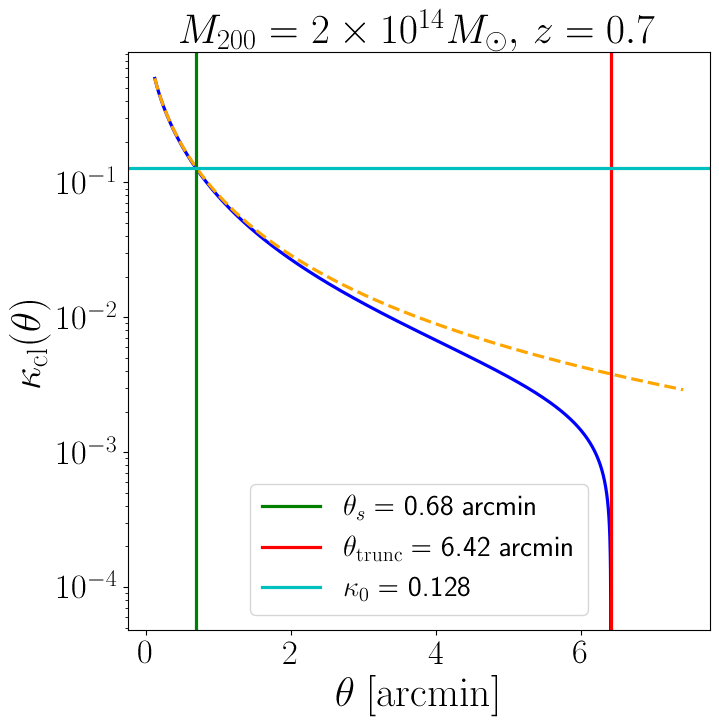
\includegraphics[width=0.7\hsize]{Figures/template_func_theta_.png}}
   %\subfigure[ ]{
   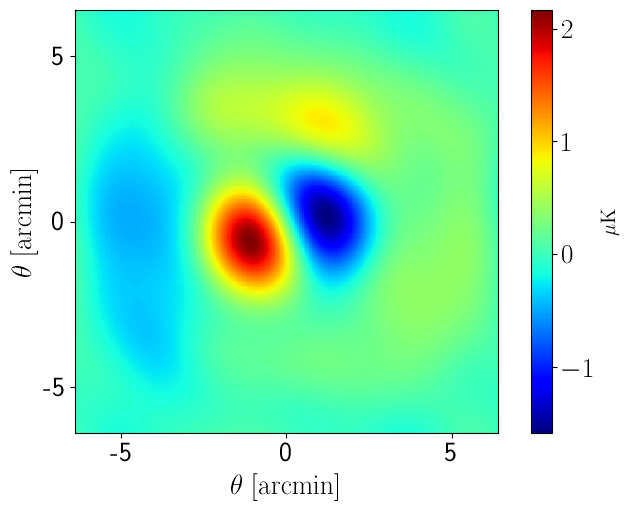
\includegraphics[width=0.85\hsize]{Figures/cluster_dipole.png}%}
   \caption{This figure \JC{No need of 'this plot, this figure, etc...'} shows the well-known dipole-like structure that we expect in (lensed-unlensed)~\protect\footnotemark[1] sky when there is a cluster with $M_{200} = 2\times 10^{14} M_{\odot}$\protect\footnotemark[2], $z=0.7$ present in our line of sight.}
   \label{fig:dipole} 
\end{figure}

 
Here, $\kappa_t$ is a circularly symmetric template function, which has a functional dependence on $\frac{r}{r_s}=\frac{\theta}{\theta_s}$. The normalisation $\kappa_0$ is chosen such that $\kappa_t = 1$ at scale radius and the cluster convergence is $\kappa_0$ there.\footnotetext[1]{The simulations have been obtained using our code LensIt: \url{https://github.com/carronj/LensIt}}\footnotetext[2]{$M_{\odot}$ is the solar mass, i.e. $1.99\times 10^{30}$ kilogram} When there is such a circularly  symmetric convergence profile in front of a temperature gradient, we expect a dipole-like structure in the lensed-unlensed CMB~\cite{Seljak:1999zn}, as depicted in Figure~\ref{fig:dipole}. Given the definition of $\kappa_0$, it has direct proportionality relation with the mas of the cluster $M_{200}$ \cite{Zubeldia:2019brr},
\begin{equation}\label{eq:tracer}
    \kappa_0 \theta_s^2 \propto \frac{M_{200}}{\Sigma_{\text{crit}}(z)d_{A}^2(z)}
\end{equation}
Hence, $\kappa_0$ works as tracer of the cluster mass and constraining the signal to noise ratio (SNR) for $M_{200}$ boils down to constraining the same quantity for $\kappa_0$, $\frac{\sigma_{\kappa_0}}{\kappa_0} = \frac{\sigma_{M_{200}}}{M_{200}}$. 

Since the convergence profile is circularly symmetric, we can use standard simplifications in Fourier space, as follows
\begin{equation}\label{eq:FT1}
    \kappa(\ell) = \int d^2 \theta\: \kappa(\theta) e^{- i \bs{\ell}\cdot\bs{\theta}} = 2\pi \int_0^{\infty} d\theta \: \theta \kappa(\theta) J_0(\theta \ell)
\end{equation}
Here $J_0$'s are first kind Bessel's function of zeroth order. We can use the asymptotic approximation of the Legendre Polynomial, i.e. $P_\ell(\cos \theta) \underbrace{\rightarrow}_{\ell \rightarrow \infty} J_0(\ell \theta)$ to express the above expression as the spin 0 Wigner transform of the convergence profile.
\begin{equation}\label{eq:FT2}
    \kappa(\ell) \sim 2\pi \int_{-1}^1 d \cos (\theta )\:\kappa(\theta) P_\ell(\cos \theta)
\end{equation}
The transform is also circularly symmetric in 2D Fourier space. The analytical form of the Fourier transform has been provided in Appendix~\ref{A2}. \JC{I would put this and 2.12 in appendix and just keep here the non-technical discussion that leads to the template function etc}


\section{Cluster mass estimators}
\label{sec:method}

\subsection{Lensing Reconstruction}
% The most conventional lensing estimate present in the literature is the quadratic estimator \cite{Hu:2001tn, Hu:2001kj, Okamoto:2003zw}. The weak lensing phenomena breaks the statistical isotropic nature of the primordial CMB fluctuations and couples different multipoles in the Fourier space. 
% The quadratic estimator basically uses this strength of coupling in the observed CMB temperature of polarisation maps to estimate the lensing potential or convergence. At the current noise level, the quadratic estimators are nearly fine. In light of future experiments, such as CMB-S4 \cite{CMB-S4:2016ple, CMB-S4:2022ght}, where temperature noise level is as low as 1 $\mu$K-arcmin and polarisation noise level is 1.4 $\mu$K-arcmin, the quadratic estimators are sub-optimal, as the lensing B modes kicks in. 

\LL{TODO: homogenize notations with the previous section}

We work in the flat sky approximation, and identify multipoles to the plane wave vectors $\vell = (\ell_x, \ell_y)$, and use the symmetric Fourier transform convention\JC{x, really?}
\begin{equation}
    x(\vell) = \int \frac{d^2 \vn}{2\pi} x(\vn) e^{-i\vell \vn}\, ,
\end{equation}
which we write in the compact notation $x(\vell) = \mathcal{Y} x(\vn)$.
As standard in literature, we use $\vell$ for the CMB multipoles and $\vL$ for the lensing multipoles.   

Let $X$ be the unlensed CMB temperature or polarisation field, $X \in \{T, E, B\}$, expressed in Fourier space. 
The covariance of these unlensed fields are the primordial power spectra 
$\left<X_{\vell}, X_{\vell'}^\dagger \right> = \delta^{\ell}_{\ell'} C_\ell^{\rm unl}$.

The observed CMB field in pixel space can be expressed as 
\begin{equation}
    X^{\rm dat} = BDX + n
\end{equation}
where $D$ is the operator that maps the unlensed CMB modes to the lensed CMB in real space (and thus contains the $\mathcal{Y}$ operator). The operator $B$ is the linear response matrix of the instrument, including beam and pixel window functions, and $n$ is an independent noise, expressed in pixel space. 
For a given deflection filed the covariance of the observed CMB fields is
\begin{equation}
    \Cov_{\valpha} \equiv \left<X^{\rm dat} X^{\rm dat, \dagger} \right>_{\valpha}  = BDC^{\rm unl} D^\dagger B^\dagger + N \, ,
\end{equation}
where $N$ is the noise covariance matrix in pixel space. 
While if averaging on the deflection fields as well we can write this covariance as 
\begin{equation}
    \Cov \equiv \left<X^{\rm dat} X^{\rm dat, \dagger} \right> = B \mathcal{Y} C^{\rm len} \mathcal{Y}^\dagger B^\dagger + N \, ,
\end{equation}
where $C^{\rm len}$ is the covariance of the lensed CMB fields, given by the fiducial lensed CMB power spectra. 

In pixel space, the unnormalized quadratic estimator of the lensing deflection field can be expressed as the product of two filtered CMB maps\JC{is minus sign right here ?}
\begin{equation}\label{Eq:QE}
    \hat \valpha^{\rm QE}(\vn) = - \bar X(\vn) \, \grad X^{\rm WF}(\vn) \, ,
\end{equation}
where the inverse variance filtered and Wiener filtered legs are
\begin{equation}
    \begin{split}
        \bar X &= B^{\dagger} \Cov^{-1} X^{\rm dat} \, , \\
        X^{\rm WF} &= C^{\rm len}  \mathcal{Y}^\dagger B^{\dagger} \Cov^{-1} X^{\rm dat} \, .
    \end{split}
\end{equation}
The normalisation of the QE is chosen to obtain an unbiased estimator, and is expressed in Fourier space as $N(\vL)$ \cite{Hu:2001kj}. \JC{better use response language}
This gives the normalised QE convergence field in Fourier space\JC{$\valpha^{\rm QE}_\vL$ instead of $\mathcal Y \hat \valpha^{\rm QE} $?}
\begin{equation}
    \hat \kappa^{\rm QE}(\vL) = \frac{2}{\vL^2} N(\vL) \, \mathcal{Y} \, \hat \valpha^{\rm QE} \, .
\end{equation}

The maximum a posteriori estimator finds the deflection field that maximize the likelihood of the lensed CMB fields, assuming a Gaussian prior on the lensing potential, with power spectrum $C_L^{\phi\phi, \rm fid}$
\begin{equation}
    \ln \mathcal{P}(\valpha | X^{\rm dat}) = \ln \mathcal{L}( X^{\rm dat} | \valpha) - \frac{1}{2} \, \sum_\vL \frac{\phi_\vL \phi_{\vL'}^\dagger}{C_L^{\phi\phi, \rm fid}}
\end{equation}
where the lensed CMB likelihood is assumed to be Gaussian and given by 
\begin{equation}
    \ln \mathcal{L}( X^{\rm dat} | \valpha) = -\frac{1}{2} X^{\rm dat, \dagger }\Cov_\valpha^{-1} X^{\rm dat} - \frac{1}{2}\ln \det \Cov_\valpha
\end{equation}
In practice, the MAP lensing deflection field $\valpha^{\rm MAP}$ is found by Newton-Raphson iterations on the posterior, until convergence. Each iteration step can be obtained by running a QE with modified weights on partially delensed CMB maps  \cite[see][for more details]{Carron:2017mqf}.

The normalisation of this estimator is however not tractable analytically. We follow \cite{Legrand:2021qdu,Legrand:2023jne} and obtain an empirical normalisation of our MAP estimator from a set of simulations\JC{a tiny bit more details on how you do that might be in order here,  a sentence, or one equation}. As shown in \cite{Legrand:2021qdu,Legrand:2023jne}, this empirical normalisation is not sensitive to the cosmology or to the noise level, allowing for a robust normalisation even when the true cosmology and noise statistics are poorly known.  

\JC{Plus some comment here on deflection-inversion and finufft changes}
\subsection{Cluster Signal Reconstruction}
Once we have the lensing reconstruction from observed CMB, we want to fit our theoretical template $\kappa_0\kappa^t (\bs\ell)$ to those observations $\hat \kappa (\bs\ell)$ with a Gaussian noise $N(\bs\ell)$, i.e. $\langle{\hat\kappa (\bs\ell) \hat\kappa (\bs\ell')}\rangle -  \langle{\hat \kappa (\bs\ell)}\rangle \langle \hat \kappa (\bs{\ell}') \rangle = \delta(\bs\ell - \bs\ell') N (\bs\ell)$. We can construct a minimum variance estimator of $\kappa_0$ as a function of the lensing estimation $\hat{\kappa}$ of the observed map. 

\begin{figure*}
  \subfigure[ ]{
  \label{fig:kappa_th}
  \hspace*{-1.0cm}
  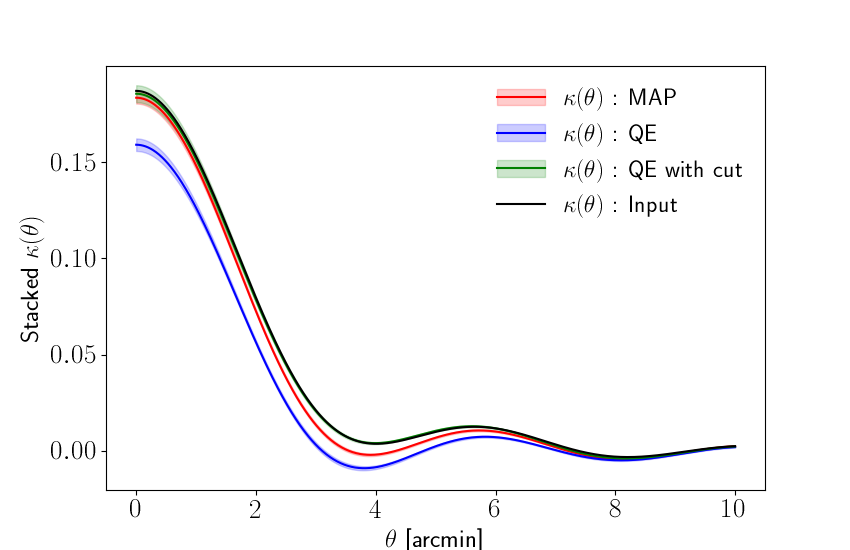
\includegraphics[width=0.55\hsize]{Figures/kappa_thet_lmax5k_out5k_M4.png}}
  \subfigure[ ]{
   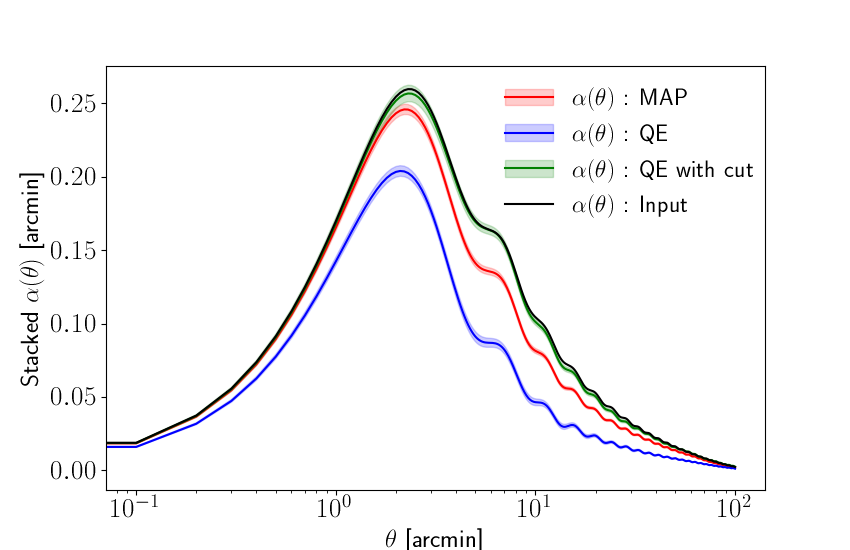
\includegraphics[width=0.55\hsize]{Figures/alpha_thet_lmax5k_out5k_M4.png}}
\caption{These plots depict the stacking of reconstructed $\kappa$ and $\alpha$ profiles from a set of $1000$ simulations. In this analysis, we evaluate the performance of various estimators and compare their results with the input data. To recover the profile in real space, we employ multipoles up to $\ell_{\text{max}} = 5000$.\JC{better caption}}
\label{fig:Bias_sup}
\end{figure*}

\begin{equation}\label{eq:kappa_0}
    \hat{\kappa}_0 = \frac{\int \frac{d^2\vecell}{(2\pi)^2}  \frac{\kappa^t(\vecell) \hat \kappa(\vecell)}{N(\vecell)}}{\int\frac{d^2\vecell}{(2\pi)^2}  \frac{|\kappa^t(\vecell)|^2}{N(\vecell)}}.
\end{equation}
Due to symmetry of the problem as shown in the previous section, all the quantities in the above expression are function $\ell = |\bs\ell|$. Hence the \JC{theoretical} error \JC{$\sigma^2$}for the above estimator is given as follows,
\begin{equation}\label{eq:kappa_0_noise}
    \frac{1}{\sigma^2} = \frac{1}{2\pi}\int d\ell\: \ell \frac{|\kappa_t(\ell)|^2}{N(\ell)} 
\end{equation}
In these equations, the noise of the $\hat \kappa(\ell)$ estimate is, $N(\ell) = C_\ell^{\kappa\kappa} + N_0(\ell) + N_1 (\ell)$. The $C_\ell^{\kappa\kappa}$ is the power spectrum of the background convergence profile of the large scale structure (LSS), which should be treated as a Gaussian noise in context of the lensing signal from clusters\JC{plus one comment on clusters being part of LSS}. The $N_0 (\ell), N_1(\ell)$ are known $N_0$ and $N_1$ biases in the literature \cite{Kesden:2003cc,Lewis:2006fu}.\JC{One more sentence to describe the difference between the two}

In the following section, we present the forecast of our mass estimator based on MAP (Maximum A Posteriori) methodology. Additionally, we delve into the outcomes obtained by applying this estimator on simulations.

\section{Results}
\label{sec:results}

To estimate the mass of the cluster, we employ matched filtering, as described by Eq. \ref{eq:ft_anal1} and \ref{eq:ft_anal2}. We demonstrate the application of both the quadratic estimator and the iterative or MAP estimator, as explained in the previous subsection, to obtain the estimated $\hat{\kappa}(l)$.
Our analysis focuses on a CMB S4-like experiment, where the forecasted noise level is a few\JC{??} $\mu K$-arcmin. We assume a beam with a full width at half-maximum (FWHM) of 1 arcmin and use a pixel size of $0.3$ arcmin. Simulations of a sky patch with $N_{\text{side}}=1024$\JC{Nside not a good name here, confusing with healpy Nside} are used for our analysis. To simplify the calculations, we employ the flat-sky approximation.
In the first part of this section, we examine the low bias in temperature caused by moderate to strong lensing in the cluster center. In the second part, we present the results of our estimator, along with the corresponding theoretical forecast, assuming that $M_{200}$ is $2\times10^{14} M_{\odot}$ and $z$ is $0.7$.
\subsection{Bias in Temperature QE}
As discussed in the literature \cite{Hu:2007bt, Maturi:2004zj, Amblard:2004ih}, the temperature quadratic estimator is biased low due to strong to moderate lensing close to the cluster center. As the strong lensing magnifies the background CMB, it seems \JC{seems or does?}to decrease the gradient of the background CMB to the weak-lensing QE. Since the weak lensing signature, i.e. the dipole-like structure in the lensed-unlensed sky, is sensitive to both the strength of the gradient and the mass of the cluster, it decreases that signature as well. As a consequence, when we estimate cluster signal using weak lensing temperature QE, the estimator is biased low. 

The temperature quadratic estimator is nothing but a product of two filtered maps as given in Eq.~\ref{Eq:QE}. The bias comes mainly from the small scales in the gradient leg. A solution to this bias, as demonstrated in \cite{Hu:2007bt}, is to use a low-pass filter for the gradient leg and only include multipoles below $\ell=2000$. In Appendix~\ref{A1}, we present the analytical forecast on the performance of such modified QE compared to conventional QE in the context of the bias\JC{??}. In this section we present how our MAP estimator perform on simulations and compare it with the QE's. Since the bias is more prominent for massive clusters and small scales, we choose the clusters parameters to be $M_{200} = 4 \times 10^{14} M_{\odot}, z=0.7$ and use CMB multipoles from $\ell_{\text{min}}^{\text{CMB}}=100$ to $\ell_{\text{max}}^{\text{CMB}} = 5000$ for this section. We run all the estimators on $1000$ simulations and stack the reconstructed maps and compare it with the input cluster signal. We also subtract the noise of the reconstruction to eliminate the variance of the noise due to stacking. In Figure~\ref{fig:Bias_sup}, we provide the comparison for the deflection profile, $\alpha(\theta)$  and the convergence profile $\kappa (\theta)$. Although, $\alpha$ and $\kappa$ is reconstructed in 2D patch, we bin the polar angle to get an one dimensional plot as a function of radius (or angular distance from the centre) of those quantity. The deflection $\alpha$, which is the gradient of the lensing potential $\phi$ is a vector quantity. But it only has the non-zero radial component, since cluster is circularly symmetric. Hence we only binned radial component of $\alpha$. As expected the QE is biased low for such massive clusters, whereas the modified QE~\cite{Hu:2007bt} with the cut in the gradient leg does almost unbiased reconstruction of the cluster signal. Our iterative estimator in other hand, does manage to get rid of the bias up to some limit\JC{Must quantify this}, without wasting any information in the small scale regime\JC{how much was wasted with cut?}. Therefore, in the next section, we discuss how the iterative estimator also suppresses the noise of the mass estimation compared to QE. We refer to the modified QE as QE \JC{hmm} for the temperature estimator from now on.
\begin{figure}
    \centering
    \hspace*{-1.0cm} 
    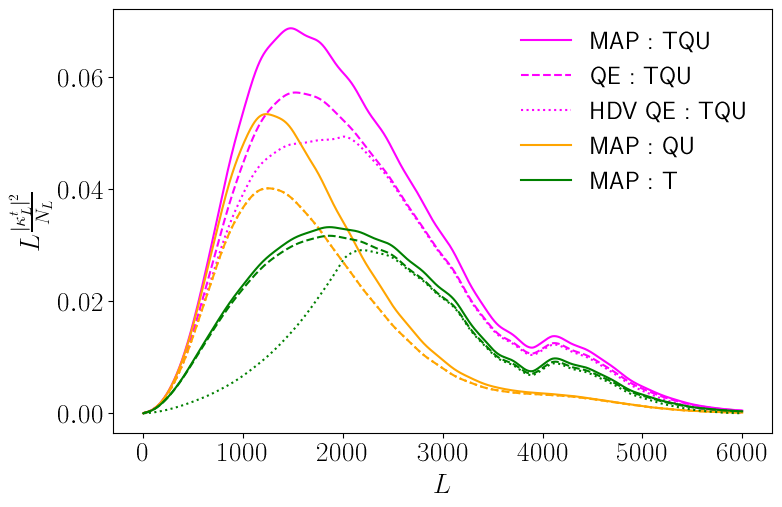
\includegraphics[width=1.\hsize]{Figures/Integrand.png}
    \caption{This figure plots the integrand in Eq.~\ref{eq:kappa_0_noise}, which depicts the relevant scales, while estimating cluster signal from reconstructed $\hat{\kappa}$ using different estimator}
    \label{fig:int}
\end{figure}
\subsection{\JC{CMB fluctuation?}Noise suppression}
As we have discussed in the Introduction, the conventional QE is sub-optimal when the noise level is few $\mu K$-arcmin. Here we present the comparison of noise in the mass estimation QE and iterative estimator. We present the theoretical forecast on noise using Eq.~\ref{eq:kappa_0_noise} for clusters of $M_{200} = 2\times 10^{14}, z=0.7$\JC{Why this choice?}. We used multipoles $\ell_{\text{min}}^{\text{CMB}} = 100$ to $\ell_{\text{max}}^{\text{CMB}} = 4000$ in the observed CMB to do the lensing reconstruction. For such configuration, it is important to understand which scales are important to reconstruct $\hat{\kappa}_0$ from the reconstructed $\hat{\kappa}(\ell)$. Hence in Figure~\ref{fig:int}, we plot the integrand in Eq.~\ref{eq:kappa_0_noise} for CMB-S4 noise level $\Delta T  = 1 \mu \rm{K}$-arcmin and beam FWHM$=1$ arcmin. We use $L_{\text{min}}=100$ and $L_{\text{max}}=6000$ to include information from all relevant scales for our $\hat{\kappa}_0$ calculation in Eq.~\ref{eq:kappa_0}. We use such $\ell_{\text{min}}^{\text{CMB}}$ and $L_{\text{min}}$ in our calculation, so that we include modes well inside the sky-patch. 



\begin{table}
\centering
\hspace*{1.0cm} 
\caption{\textbf{Summary of results on 1000 simulations with Input $\bs{\kappa_0 = 0.1285}$}\JC{Description missing. Fix notation of theoretical error in 3.11}}
    \begin{tabularx}{0.15\textwidth}{|X|X|}
    \hline
    \multicolumn{2}{|c|}{QE : T} \\ \hline
    $\langle\kappa_0 \rangle$      & 0.1275   \\ \hline
    $\sigma_{\kappa 0}$ & 0.0099  \\\hline
    $\sigma_{\kappa 0}^{\text{th}}$ & 0.0096  \\\hline
    \end{tabularx}
    \begin{tabularx}{0.15\textwidth}{|X|X|}
    \hline
    \multicolumn{2}{|c|}{QE : QU} \\ \hline
    $\langle\kappa_0 \rangle$      & 0.1397   \\ \hline
    $\sigma_{\kappa 0}$ & 0.0088  \\\hline
    $\sigma_{\kappa 0}^{\text{th}}$ & 0.0090  \\\hline
    \end{tabularx}
    \begin{tabularx}{0.15\textwidth}{|X|X|}
    \hline
    \multicolumn{2}{|c|}{QE : TQU} \\ \hline
    $\langle\kappa_0 \rangle$      & 0.1309   \\ \hline
    $\sigma_{\kappa 0}$ & 0.0064  \\\hline
    $\sigma_{\kappa 0}^{\text{th}}$ & 0.0067  \\\hline
    \end{tabularx} \\ 
    \begin{tabularx}{0.15\textwidth}{|X|X|}
    \hline
    \multicolumn{2}{|c|}{MAP : T} \\ \hline
    $\langle\kappa_0 \rangle$      & 0.1272   \\ \hline
    $\sigma_{\kappa 0}$ & 0.0082  \\\hline
    $\sigma_{\kappa 0}^{\text{th}}$ & 0.0083  \\\hline
    \end{tabularx}
    \begin{tabularx}{0.15\textwidth}{|X|X|}
    \hline
    \multicolumn{2}{|c|}{MAP : QU} \\ \hline
    $\langle\kappa_0 \rangle$      & 0.1342   \\ \hline
    $\sigma_{\kappa 0}$ & 0.0078  \\\hline
    $\sigma_{\kappa 0}^{\text{th}}$ & 0.0081  \\\hline
    \end{tabularx}
    \begin{tabularx}{0.15\textwidth}{|X|X|}
    \hline
    \multicolumn{2}{|c|}{MAP : TQU} \\ \hline
    $\langle\kappa_0 \rangle$      & 0.1331   \\ \hline
    $\sigma_{\kappa 0}$ & 0.0061  \\\hline
    $\sigma_{\kappa 0}^{\text{th}}$ & 0.0062  \\\hline
    \end{tabularx}
    \label{tab:results}
\end{table}

In Table~\ref{tab:results}, we provide the summary of our results using the estimators on simulations along with the forecast on noise for those estimator. We also plot those results along with the forecast of mass estimation in Figure~\ref{fig:forecast}.   
\begin{figure}[H]
    \centering
    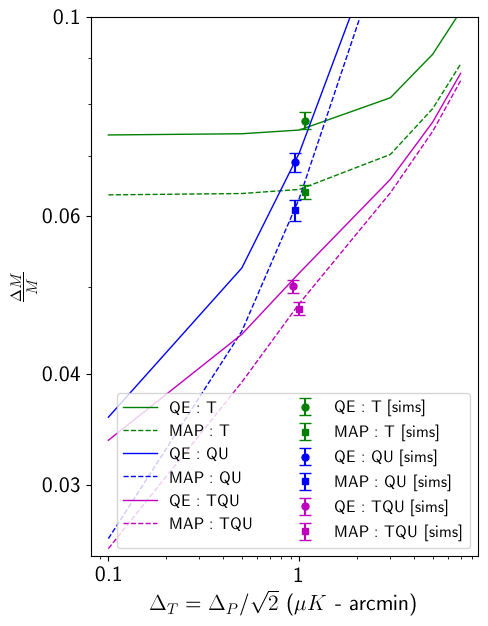
\includegraphics[width=1.\hsize]{Figures/forcast_snr.png}
    \caption{In this plot, the solid and dashed lines represent the theoretical forecasts of Inverse Signal-to-Noise Ratio (SNR)\JC{ISNR ...?} for QE and MAP, respectively. The parameters used are $M_{200} = 2\times10^{14}M_{\odot}$ and $z=0.7$, with a range of noise levels in units of a few $\mu K$-arcmin. The beam FWHM is $1$ arcmin. The error bars indicate the results obtained from 1000 simulations conducted with a noise level of $1 \mu \rm{K}$-arcmin.}
    \label{fig:forecast}
\end{figure}

As mentioned in the previous section, we employ the modified QE~\cite{Hu:2007bt} for the temperature estimator, referred to as `QE : T' in this section. With the noise level of the CMB S4, the MAP estimator detects the cluster signal with a significance of $21.8\sigma$, representing an approximate $5\%$ \JC{?? how was this calculated ?}enhancement compared to QE. While our results are presented based on 1000 simulations, they can be extrapolated to the projected number of clusters in CMB S4, estimated to be $10^5$. In our analytical forecasts and the estimation on simulations, we have included the lensing of CMB from the large scale structure (LSS) as well. In the context of cluster-lensing, it is accounted as a Gaussian noise. Although the LSS-lensing is supposed to vanish due to stacking of sky-patches, it still contributes to the noise of lensing reconstruction. Hence, it is important to account for the LSS lensing and all the complicacy that comes with it. It is worth noting that in both our analytical forecasts and simulations, we accounted for the lensing effects of the large-scale structure (LSS) on the CMB. In the realm of cluster-lensing, the LSS lensing is treated as Gaussian noise. Despite efforts to mitigate its impact through stacking of sky-patches, the LSS lensing still contributes to the noise in the lensing reconstruction process. Thus, it is crucial to consider the influence of LSS lensing and all the associated complexities it brings.
%We expect $10^5$ number of clusters to be detected for S4 experiment. We provide the forecast on Inverse signal to noise ratio (SNR) for $10^5$ for conventional QE and MAP estimator in figure and we show the improvement in figure . We consider modes from $\ell_{min}=100$ to $\ell_{max}=4000$ in the lensed CMB maps for estimating $\hat \kappa (\ell)$ in both cases.

%\begin{figure}[H]
%   \centering
%   \subfigure[ ]{
%   \label{fig:snr_4k}
   %\hspace*{-1.4cm}
%   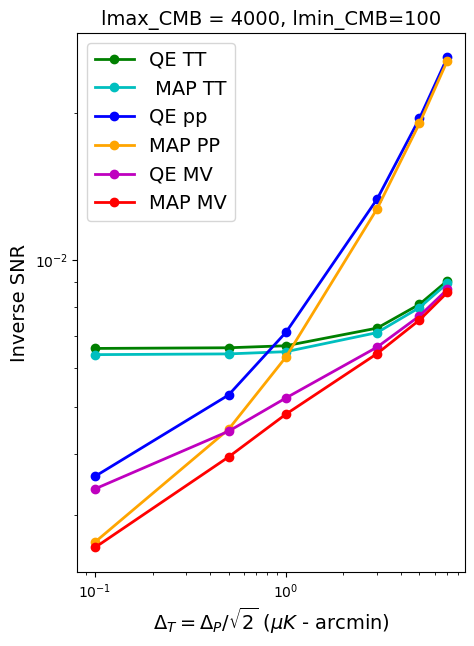
\includegraphics[width=0.7\hsize]{Figures/snr_forecast_lmax4k.png}}
%   \subfigure[ ]{
%   \label{fig:improvement}
%   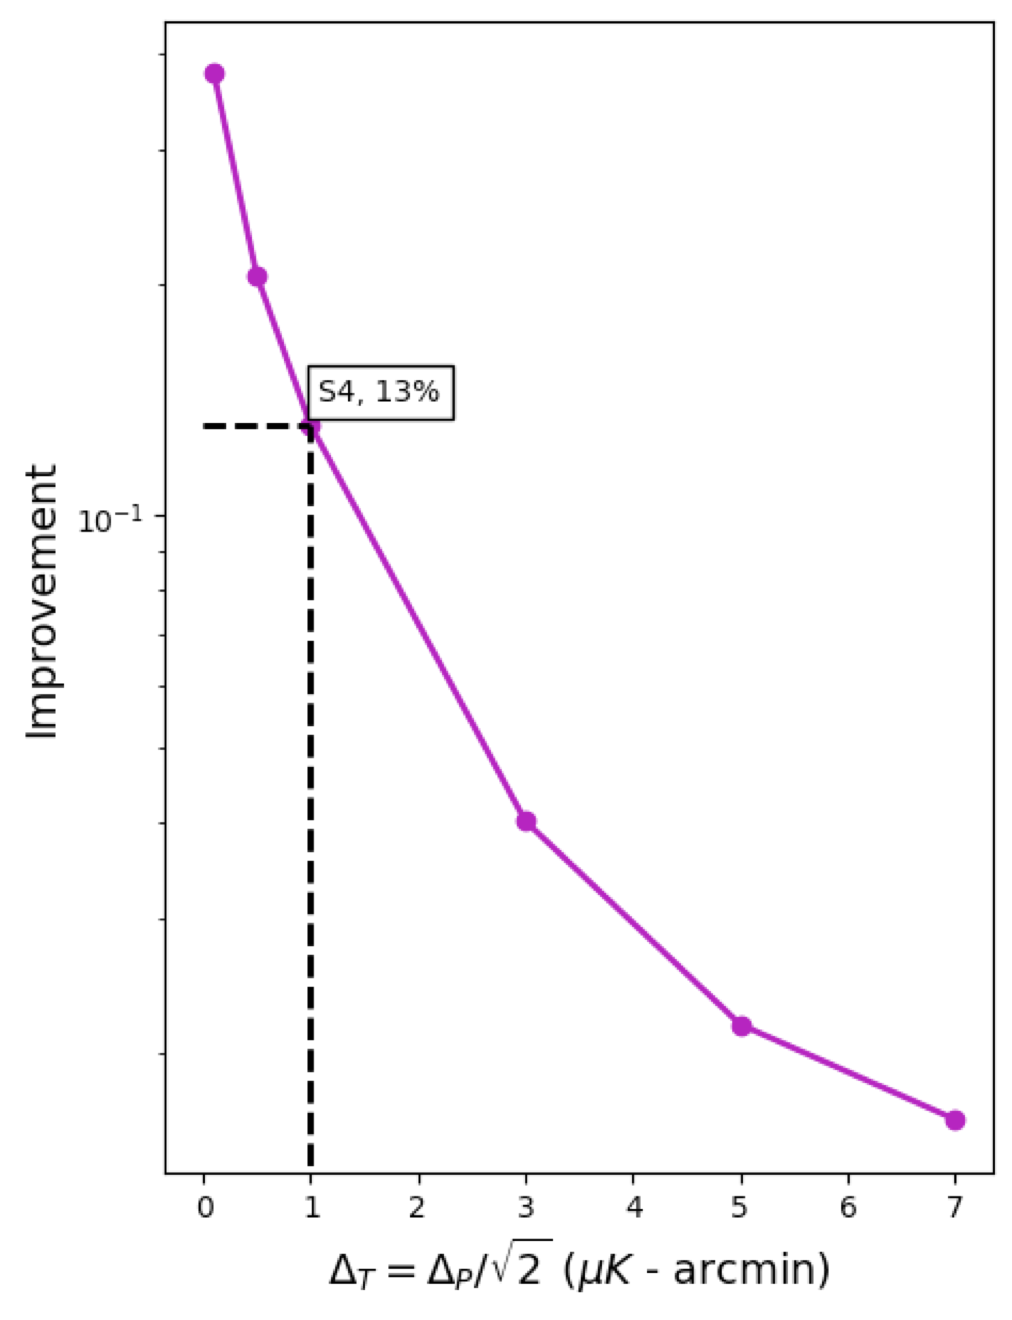
\includegraphics[width=0.7\hsize]{Figures/improvement_lmax4k.png}}
%   \caption{}
%\end{figure} 

\section{Conclusions}
\label{sec:conclusion}

In this study, we have conducted an investigation into the phenomenon of CMB lensing by galaxy clusters, with a particular focus on utilizing this process to reconstruct the mass profile of the clusters. To address the inherent challenges associated with this task, we have introduced the maximum a posteriori (MAP) estimator~\cite{Carron:2017mqf} as a novel approach for accurately estimating the convergence $\kappa$ in the context of cluster lensing.

A primary concern we have addressed pertains to the bias observed in the temperature quadratic estimator (QE) when strong to moderate lensing occurs near the central region of the cluster. While the modified QE successfully mitigates this bias, it introduces additional noise due to the underutilization of information at small scales. Conversely, our findings indicate that the MAP estimator offers improved performance over the QE approach by effectively reducing the bias without compromising information extraction at small scales. Consequently, the MAP estimator emerges as an appealing choice for the task of reconstructing cluster masses.

In the subsequent section of our study, we have quantitatively assessed the performance of the MAP estimator in the presence of CMB S4 noise. By considering a sample size of $1000$ clusters, we report a highly significant detection of the cluster signal with the MAP estimator, reaching a level of $21.8\sigma$. Notably, this represents an approximate $5\%$ improvement in detection significance compared to the QE approach. These outcomes underscore the robustness and precision of the MAP estimator in the realistic observational context of cluster signal detection.

In summary, our study demonstrates the efficacy of the MAP estimator in mitigating bias and enhancing the accuracy of mass estimation in the realm of cluster lensing. Through a rigorous comparison with the QE approach, we have substantiated the distinct advantages offered by the MAP estimator in addressing bias while fully utilizing available information. These findings contribute to the advancing body of knowledge concerning CMB cluster lensing and provide valuable insights for future investigations focused on the reconstruction of galaxy cluster mass profiles through the exploitation of CMB lensing techniques.
\JC{mention tough aspects like calculation of WF}

\begin{acknowledgements}
The authors acknowledge helpful discussions with Mathew Madhavacheril and Sebastian Belkner. SS acknowledges support from the Federal Commission for Scholarships for Foreign Students for the Swiss Government Excellence Scholarship (ESKAS No. 2022.0316) for the academic year 2022-'23.
\end{acknowledgements}
%\onecolumngrid
\bibliography{CL}
\appendix
\section{Theoretical Expressions in Clusters Lensing}\label{A2}
The expression for the convergence profile of the galaxy clusters is given by~\cite{Takada:2002qq},
\begin{equation}
    \kappa_{cl} = \frac{2\rho_s r_s}{\Sigma_{crit}(z)}g(x), \text{ where } x=\frac{r}{r_s} = \frac{\theta}{\theta_s},
\end{equation}
and where $g(x)$ is a circularly symmetric function depending on the truncation of the profile,
\begin{equation}
    g(x) = 
     \begin{cases}
       -\frac{\sqrt{x_{\text{max}}^2-x^2}}{(1-x^2)(1+x_{\text{max}})} + \frac{1}{(1-x^2)^{\frac{3}{2}}}&\cosh^{-1}\left(\frac{x^2+x_{\text{max}}}{x(1+x_{\text{max}})}\right),  \\ &(x < 1)\\
       \frac{\sqrt{x_{\text{max}}^2 - 1}}{3(1+x_{\text{max}})}\left[ 1+\frac{1}{1+x_{\text{max}}} \right],  &(x = 1)\\
       -\frac{\sqrt{x_{\text{max}}^2-x^2}}{(1-x^2)(1+x_{\text{max}})} - \frac{1}{(x^2-1)^{\frac{3}{2}}}&\cosh^{-1}\left(\frac{x^2+x_{\text{max}}}{x(1+x_{\text{max}})}\right),  \\
       &(1< x \leq x_{\text{max}})\\
     \end{cases}
\end{equation}
The analytical form of the Fourier transform to the convergence profile, equivalent to Eq.~\ref{eq:FT1} and \ref{eq:FT2}, is given by \cite{Scoccimarro:2000gm, 2011PhRvD..83b3008O, Takada:2002qq}%in Eq 10 of \cite{Scoccimarro:2000gm}, Eq 28, 29 of \cite{2011PhRvD..83b3008O} or Eq 17 of \cite{Takada:2002qq}, but slight modification: $c_{200}$ is replaced by $x_{\text{max}}$, but the normalisation $m_{\text{nfw}}$ is always the same (depends on $c_{200}$ doesn't depend on $R_{\text{trunc}}$) 
\begin{equation}\label{eq:ft_anal1}
    \kappa_{a}(l;z) = \frac{M_{200}\Tilde{u}(k=\ell/\chi;z)}{(1+z)^{-2}\Sigma_{\text{crit}}(z)},
\end{equation}
where $\Tilde{u}(k=\ell/\chi;z)$ is given by
\begin{align}\label{eq:ft_anal2}
    \Tilde{u}(k=\ell/\chi;z) = \frac{1}{m_{\text{nfw}}}[\sin{y}\{\text{Si}[y(1+x_{\text{max}})] -\text{Si}(y)\} \nonumber \\ 
    +\cos{y}\{ \text{Ci}[y(1+x_{\text{max}})]-\text{Ci}(y) \} - \frac{\sin{(y x_{\text{max}})}}{y(1+x_{\text{max}})}].
\end{align}
Here, we define a new Fourier variable, $k =\ell/\chi$. $\chi$ is the comoving angular diameter distance at that redshift, defined as $\chi(z) = \int_0^z dz'\frac{1}{H(z')} = (1+z)d_A(z)$. In the above equation, $y = (1+z)kr_s$; $\text{Si}(x)$ and $\text{Ci}(x)$ are the sine and cosine integrals and the normalisation $m_{\text{nfw}} = \ln{(1+c_{200})}-\left(\frac{c_{200}}{1+c_{200}}\right)$.

%The analytical expression matches with Wigner transform of the profile or Fast Fourier Transform of a 2D circularly symmetric convergence profile. 


\section{Exact QE average for fixed deflection}\label{A1}
\newcommand{\hn}[0]{\hat n}
In this section we sketch how we obtain the exact expectation value of a quadratic estimator (QE) in the presence of a fixed deflection field. This allows us to predict the mass bias suffered by QE mass estimates.

We consider a generic separable temperature QE, described by two isotropic functions $F_l$ and $G_l$. Following \emph{Planck}-lensing style notation, it may be written in configuration space,
\begin{equation}
	_{1}\hat g(\hat n) = \left( \sum_{l_1m_1} F_{l_1} T_{l_1m_1}\:_sY_{l_1m_1}(\hn) \right) \left( \sum_{l_2m_2} G_{l_1} T_{l_2m_2}\:_tY_{l_2m_2}(\hn) \right) 
\end{equation}
In the case of interest, lensing, we have $s =0, t = 1$, and
\begin{equation}
	F_l = \frac{1}{C_l + N_l}, \quad G_l = - \sqrt{l(l+ 1)}\frac{C_l}{C_l + N_l},
\end{equation}
Here, $_{1} \hat g(\hat n)$ is the unnormalized deflection vector (spin-1) field estimate. We want to evaluate this quantity
\begin{equation} \label{eq:avg}
	\av{\: _{1}\hat g(\hat n)}_{\text{fixed $\phi$}},
\end{equation}
which may be used to predict the result of stacking QEs from CMB maps on identical clusters.

Let $\hat n'$ be the undeflected position that corresponds to the observed location $\hn$. Working at fixed $\hn$, by Fourier transforming the $T$-maps, we may write this as a cross-spectrum,
\begin{equation}\label{eq:g}
\begin{split}
	\av{\: _{1}\hat g(\hat n)}_{\text{fixed $\phi$}}
=\sum_{lm} C_l F^*_{lm}(\hn) G_{lm}(\hn)
 \end{split}
\end{equation}
with 
\begin{equation}
\begin{split}
    G_{lm} &= \int d^2n_2 G(\hn, \hn_2) Y^*_{lm}(\hn_2')\\
    F_{lm} &= \int d^2n_1 F(\hn, \hn_1) Y^*_{lm}(\hn_1'),
\end{split}
\end{equation}
and $F$ and $G$ have structure similar to that of a spin-weighted correlation function
\begin{equation}
\begin{split}
	F(\hn, \hn_1) &= \sum_{l_1m_1} F_{l_1} \:_sY_{l_1m_1}(\hn)\:_0Y^*_{l_1m_1}(\hn_1) \\
	G(\hn, \hn_2) &= \sum_{l_2m_2} G_{l_2} \:_tY_{l_2m_2}(\hn)\:_0Y^*_{l_2m_2}(\hn_2) \\
\end{split}
\end{equation}
For an arbitrary deflection field, this is a tough calculation, requiring several spherical harmonics transforms on non-regular grid per each point of interest $\hn$

In the case of cluster lensing things simplify quite a bit owing to
\begin{itemize}
	\item  spherical symmetry, $\av{g(\hat n)}_{\textrm{fixed deflection}}$ will depend on the co-latitude $\theta$ only, and the deflection field does not change the longitude coordinates,
	\item and the fact that clusters are small. With the coordinates such that the cluster lies at the pole, only a small number of $m$'s will be necessary. The circle at latitude $\theta$ has length $\sin \theta$, hence there is an effective $m_{\rm max} \sim l_{\rm max} \sin \theta \sim 5$ for $\theta \sim 10^{'}$ and an analysis with $l_{\rm max} = 5000$. 
	Since it is spin-1, $\av{_1g(\theta)}$ will be heavily dominated by the $m = 1$ component near the pole.
\end{itemize}
We use this to perform the calculation in Eq.~\eqref{eq:avg} by brute force, using the efficient general spherical harmonic transforms of~\cite{Reinecke:2023gtp}.

\end{document}